\chapter{Wybór narzędzi}
\qquad Przy pisaniu aplikacji tworzonej wraz z niniejszą pracą dyplomową będzie trzeba się zmierzyć z wymaganiami funkcjonalnymi i niefunkcjonalnymi określonymi w poprzednim rozdziale. Aby tego dokonać niezbędne jest wybranie odpowiednich narzędzi, które pomogą w ich realizacji. W dalszej części rozdziału zaprezentowano uzasadnienie wyboru konkretnych składowych tworzonego systemu.

Językiem programowania wybranym do napisania tej części aplikacji jest Java. Jest to język, który charakteryzuje niezależność od systemu operacyjnego i procesora. Uniwersalny kod kompilowany jest do kodu bajtowego i następnie wykonywanego przez maszynę wirtualną Javy. 

W wersji 8 tego języka, która w 2018 roku była najczęściej wybierana jako wersja do tworzenia dużych systemów komercyjnych [20], dodano wiele udogodnień pozwalających na cześciowe pisanie kodu w myśl paradygmatu programowania funkcyjnego dzięki wprowadzonym operacjom na strumieniach i wyrażeniom lambda. Java swoją popularność zawdzięcza także wykorzystaniu do tworzenia aplikacji webowych, której przykładem jest aplikacja tworzona na potrzeby tej pracy. Język ten cały czas się rozwija. Przygotowywana jest obecnie 12. wersja Javy, która ma być dostępna w marcu 2019 roku. Przykład zastosowania operacji na strumieniach oraz wyrażenie lambda przedstawiono na rysunku 5.1..

\begin{figure}[h] % h means here
	\centering
	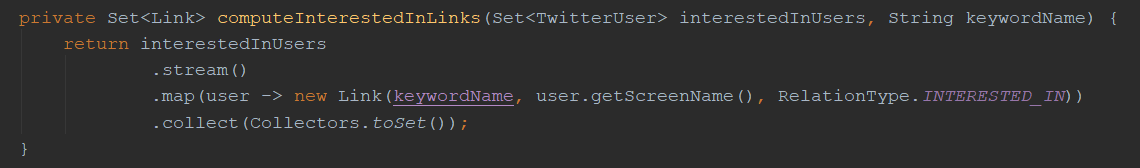
\includegraphics[width=1.0\linewidth]{img/tools_java_1}
	\caption{Przykład zastosowania operacji na strumieniach oraz wyrażenia lambda w kodzie napisanym w języku \textit{Java} w wersji 8 [materiały własne].}
\end{figure}

Jedną z bibliotek użytych w aplikacji jest biblioteka Lombok, która jest bardzo pomocna przy pisaniu prostych i powtarzalnych części kodu takich jak np. konstruktory, akcesory, mutatory, czy metody equals i hashCode. Przykładowo żeby napisać konstruktor posiadający jako argumenty wszystkie pola klasy wystarczy dodać na klasie adnotację \textit{@AllArgsConstructor} co zaprezentowano na rysunku 5.2.. Lombok jest rozwijaną bibliteką typu open-source. Jest bardzo przydatna w podstawowych potrzebach kodu pisanego w Javie.  

\begin{figure}[h] % h means here
	\centering
	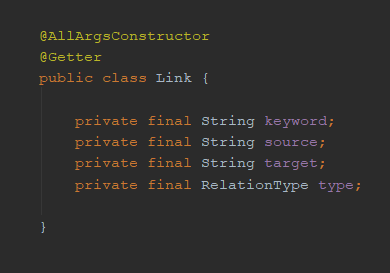
\includegraphics[width=0.6\linewidth]{img/tools_lombok_1}
	\caption{Przykład zastosowania adnotacji biblioteki \textit{Lombok} [materiały własne].}
\end{figure}

Językiem programowania wybranym do napisania części prezentacji przygotowywanej aplikacji jest JavaScript. Język ten znajduje swoje zastosowanie w tworzeniu stron internetowych. Umożliwia reagowanie na zdarzenia wywołane w przeglądarce oraz wyświetlanie efektownych efektów wizualnych. 

Dodatkowo w części front-end zostanie użyta biblioteka \textit{React.js}, która jest określana jako \textit{silnik do budowy interfejsów użytkownika} [21]. React.js charakteryzuje się wykorzystaniem reaktywnego renderowania, które polega na przechowywaniu w pamięci reprezentacji struktury DOM i ponowne renderowanie interfejsu użytkownika tylko w tych miejscach, które zależą od zmienionego stanu. Jest to biblioteka bardzo wydajna i szybka co będzie bardzo pomocne przy budowie aplikacji.

Frameworkiem, na którym opierać się będzie tworzony system jest \textit{Spring Boot}. \textit{Spring Framework} jest określany jako główna platforma programistyczna, która sprawia, że programowanie w języku Java staje się łatwiejsze i bardziej wydajne. Spring Boot natomiast opiera się na zasadzie działania Spring Framework, ale rozwiązuje wiele problemów wynikających z potrzeby konfiguracji projektu przed rozpoczęciem implementowania nowych funkcji. Posiada zbiór wszystkich wymaganych bibliotek oraz konfiguracji zwanych \textit{starterami} oraz wbudowany serwer aplikacyjny Tomcat. Spring jest bardzo dobrze udokumentowanym frameworkiem używanym przez programistów w wielu bardzo zróżnicowanych systemach.

Narzędziem wybranym do przetwarzania danych strumieniowych będzie \textit{Apache Spark Streaming}, które charakteryzuje się łatwością integracji oraz operowaniem na kolekcjach informacji zamiast pojedynczych wiadomościach. Rozwiązanie to opiera się o \textit{RDDs} - \textit{Resilient Distributed Datasets} reprezentujące kolekcje rekordów, na których można wykonywać operacje znane z paradygmatu programowania funkcyjnego np. \textit{map}, \textit{filter}, \textit{groupByKey} i \textit{join} [22]. Spark Streaming z definicji operuje na każdej porcji danych dokładnie raz. W bardzo rzadkim przypadku wystąpienia błędu może się zdarzyć, że dane nie zostaną przetworzone ani razu. Wówczas zostaną utracone dane z jednego okna czasowego trwającego kilka sekund co w kontekście budowanego rozwiązania wydaje się być dopuszczalne. Spark Streaming dobrze integruje się z językiem Java i frameworkiem Spring. Schemat zasady działania Apache Spark znajduje się na rysunku 5.3..

\begin{figure}[h] % h means here
	\centering
	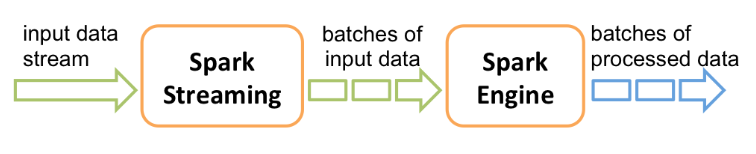
\includegraphics[width=1.0\linewidth]{img/tools_apache_spark_streaming_1}
	\caption{Zasada działania narzędzia \textit{Apache Spark Streaming} [21].}
\end{figure}

Systemem bazy danych wybranym do budowanego narzędzia jest \textit{neo4j}. Jest to nierelacyjny system bazodanowy, które w odróżnieniu do relacyjnych charakteryzują się brakiem narzuconego schematu modelu informacji. Umożliwia to przechowywanie różnych danych bez potrzeby zapisu ich w postaci relacji, które w przypadku większej ilości danych są bardzo kosztowne, ponieważ wymagają łączenia informacji z kilku tabel. 

Dane w neo4j przechowywane są w postaci grafów, w których węzły odpowiadają wierszom z relacyjnych baz danych, a krawędzie pomiędzy węzłami są odpowiednikiem kluczów obcych. Dzięki takim rozwiązaniom wyszukiwanie zależności między węzłami polega na poruszaniu się po grafie, a nie na kosztownym łączeniu danych. Grafowe bazy danych powstały wraz z rozwojem sieci społecznościowych, dlatego jest naturalne, że tego typu rozwiązanie zostało wybrane do budowy przygotowywanej aplikacji. neo4j dobrze integruje się z wybranymi już narzędziami. Przykład zapytania napisanego w języku Cypher wykorzystywanego przez grafową bazę neo4j zaprezentowano na rysunku 5.5..

\begin{figure}[h] % h means here
	\centering
	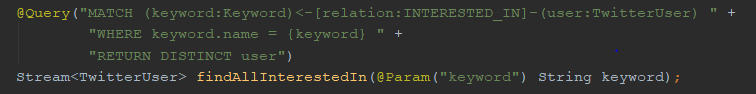
\includegraphics[width=1.0\linewidth]{img/tools_neo4j_1}
	\caption{Przykład zapytania napisanego w języku \textit{Cypher} wykorzystującego \textit{Spring Data} [materiały własne].}
\end{figure}

Biblioteką wybraną do analizy sentymentu jest rozwiązanie \textit{Stanford NLP Sentiment Analysis} tworzone i cały czas rozwijane na Uniwersytecie Stanforda. Większość dostępnych rozwiązań określa sentyment tekstu biorąc pod uwagę wydźwięk pojedynczych słów i następnie podając wynik dla całego tekstu. W ten sposób umyka informacja o kolejności wyrazów oraz zostaje zaburzony sentyment. Stanford NLP analizuje każde zdanie tekstu w całości i oblicza sentyment na podstawie tego w jaki sposób słowa składają się one na znaczenie w dłuższe zwroty [23]. 

Narzędzie to korzysta z sieci neuronowej \textit{Recursive Neural Network}, która opiera się na zasadach gramatycznych. Sieć ta została wytrenowana z wykorzystaniem zbioru recenzji filmowych zawierających prawie 12 tysięcy zdań i około 215 tysięcy słów.

Jednym z pierwszych kroków w analizie wydźwięku tekstu za pomocą tej biblioteki jest podział tekstu na zdania. Stanford NLP w swojej pełnej wersji udostępnia także parser tekstów, który może zostać użyty przy tej okazji. Następnie każde zdanie jest analizowane oddzielnie, a sentyment całego tekstu jest obliczany jako średnia arytmetyczna jego składowych. Wydźwięk podawany jest w pięciostopniowej skali: bardzo negatywny, negatywny, neutralny, pozytywny, bardzo pozytywny. Co ciekawe twórcy tego narzędzia umożliwiają na swojej stronie internetowej zwrócenie im uwagi, że pewne zdanie ze zbioru treningowego źle określa sentyment. Wówczas zostanie to przeanalizowane i poprawione. Przykład rozkładu zdania za pomocą omawionej biblioteki zaprezentowano na rysunku 5.6..

\begin{figure}[h] % h means here
	\centering
	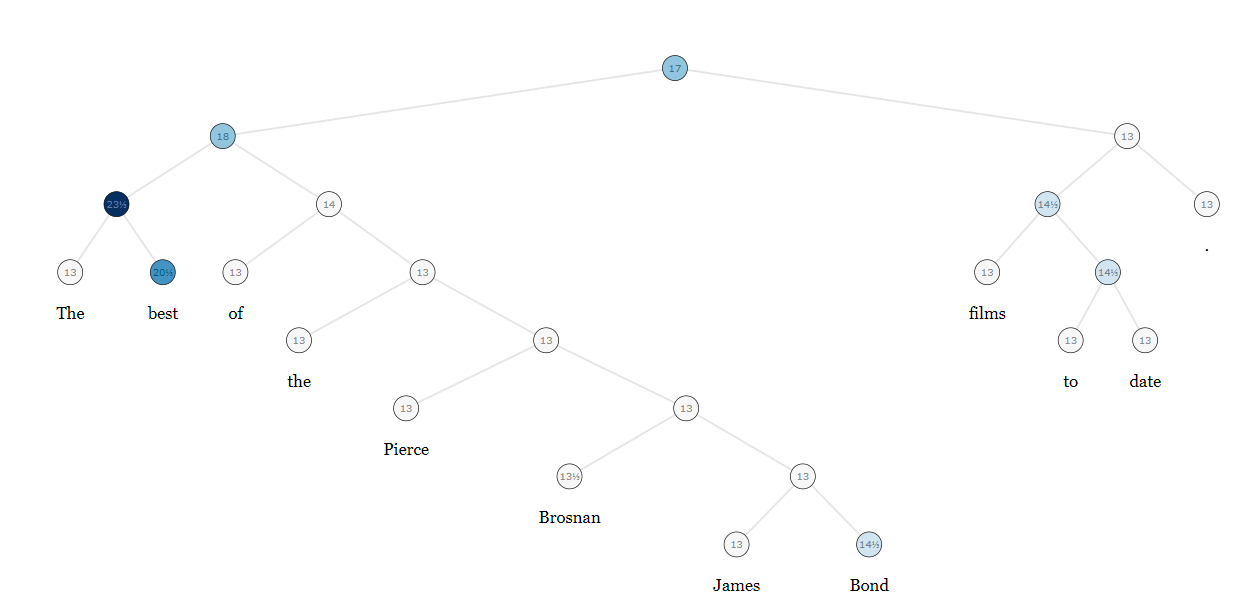
\includegraphics[width=1.0\linewidth]{img/nlp_stanford_nlp_bond}
	\caption{Przykład rozkładu opinii na temat filmu z serii \textit{James Bond} [24].}
\end{figure}

Stanford NLP wspiera obecnie badanie sentymentu tylko w tekstach angielskojęzycznych. Jego twórcy podają, że skuteczność stosowanego przez nich algorytmu wynosi 85.4\% oraz że jest to obecnie jedyne rozwiązanie, które wspiera negacje na różnych poziomach budowanych drzew w zwrotach pozytywnych i negatywnych. Narzędzie to dobrze integruje się z wybranymi już wcześniej składowymi budowanego systemu.